% This file was created by matlab2tikz.
%
\documentclass[tikz]{standalone}
\usepackage[T1]{fontenc}
\usepackage[utf8]{inputenc}
\usepackage{pgfplots}
\usepackage{grffile}
\pgfplotsset{compat=newest}
\usetikzlibrary{plotmarks}
\usetikzlibrary{arrows.meta}
\usepgfplotslibrary{patchplots}
\usepackage{amsmath}

\newlength\figureHeight \setlength{\figureHeight}{6cm}
\newlength\figureWidth \setlength{\figureWidth}{10cm}
\begin{document}
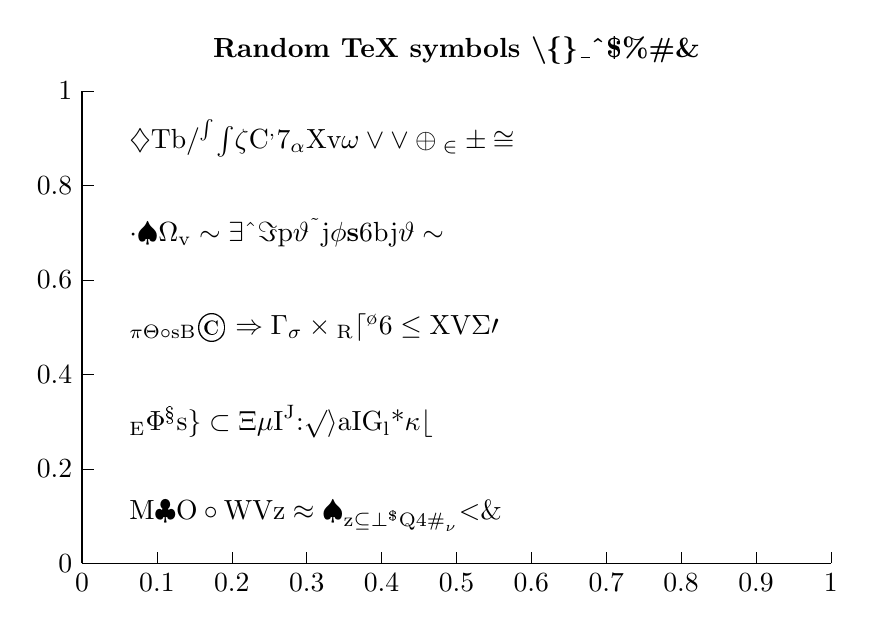
\begin{tikzpicture}

\begin{axis}[%
width=0.951\figureWidth,
height=\figureHeight,
at={(0\figureWidth,0\figureHeight)},
scale only axis,
every outer x axis line/.append style={black},
every x tick label/.append style={font=\color{black}},
every x tick/.append style={black},
xmin=   0,
xmax=   1,
every outer y axis line/.append style={black},
every y tick label/.append style={font=\color{black}},
every y tick/.append style={black},
ymin=   0,
ymax=   1,
axis background/.style={fill=white},
title style={font=\bfseries},
title={$\text{Random TeX symbols \textbackslash\{\}\_\textasciicircum\$\%\#\&}$},
axis x line*=bottom,
axis y line*=left,
legend style={legend cell align=left, align=left, draw=black}
]
\node[right, align=left]
at (axis cs:0.05,0.9) {$\diamondsuit\text{Tb/}^{\int}{\int}\zeta\text{C}^\text{,}\text{7}_\alpha\text{Xv}\omega\vee\vee\oplus{}_\in\pm{\cong}$};
\node[right, align=left]
at (axis cs:0.05,0.7) {$\cdot{\spadesuit\Omega{}_\text{v}\sim\exists\text{\textasciicircum}}\Im\text{p}\vartheta{}^\text{\textasciitilde}\text{j}{{\phi\text{\bf{}s}}\text{6bj}}\vartheta\sim$};
\node[right, align=left]
at (axis cs:0.05,0.5) {$_{\pi\Theta\circ\text{sB\bf}}\copyright\Rightarrow\Gamma{}_\sigma\times{}_\text{R}\lceil{}^\text{\o}\text{6}\leq\text{XV}\Sigma\prime$};
\node[right, align=left]
at (axis cs:0.05,0.3) {$_\text{E}\Phi{}^\text{\S}\text{s\}}\subset\Xi\mu\text{I}^\text{J}\text{:}\surd\rangle\text{aIG}_\text{l}\text{*}\kappa\lfloor$};
\node[right, align=left]
at (axis cs:0.05,0.1) {$\text{M}\clubsuit\sl\text{O}\circ\text{WVz}\approx\spadesuit{}_{\text{z}\subseteq\perp{}^\text{\$}\text{Q4\#}_\nu}\text{\textless\&}$};
\end{axis}
\end{tikzpicture}%
\end{document}